\documentclass[12pt,letter]{article}
\usepackage[moduleName=SCC]{KautenjaDSP}
% import a debugging package to show the margin boxes
% \usepackage{showframe}
% set the graphics path to the img directory
\graphicspath{{img/}}

% algorithm2e stuff
% \SetKwInOut{Objects}{$\CKmatrix{O}$}
% \SetKwInOut{Weights}{$\CKvector{w}$}

\begin{document}
\titlePage{SCC-Logo}{SCC-Module}{KautenjaDSP}
% -------------------
% MARK: Overview
% -------------------

\section*{Overview}

% SCC is an emulation of the SCC sound chip from the Nintendo Entertainment System (NES). The SCC chip contains two pulse wave generators, a quantized triangle wave generator, and a noise generator. The original chip featured a DMC loader for playing samples that has been omitted in this emulation.

% SCC provides the key features of the SCC chip, namely,
% \begin{itemize}
%   \item \textbf{Dual pulse wave generator:} Dual 8-bit pulse waves with four duty cycles: $12.5\%$, $25\%$, $50\%$, and $75\%$;
%   \item \textbf{Quantized triangle wave generator:} Generate NES style triangle wave with 16 steps of quantization;
%   \item \textbf{Noise generator:} generate pseudo-random numbers at 16 different frequencies; and
%   \item \textbf{Linear Feedback Shift Register (LFSR):} for that old-school 8-bit randomness!
% \end{itemize}

% -------------------
% MARK: Panel Layout
% -------------------

\clearpage
\section*{Panel Layout}

\begin{figure}[!htp]
\centering
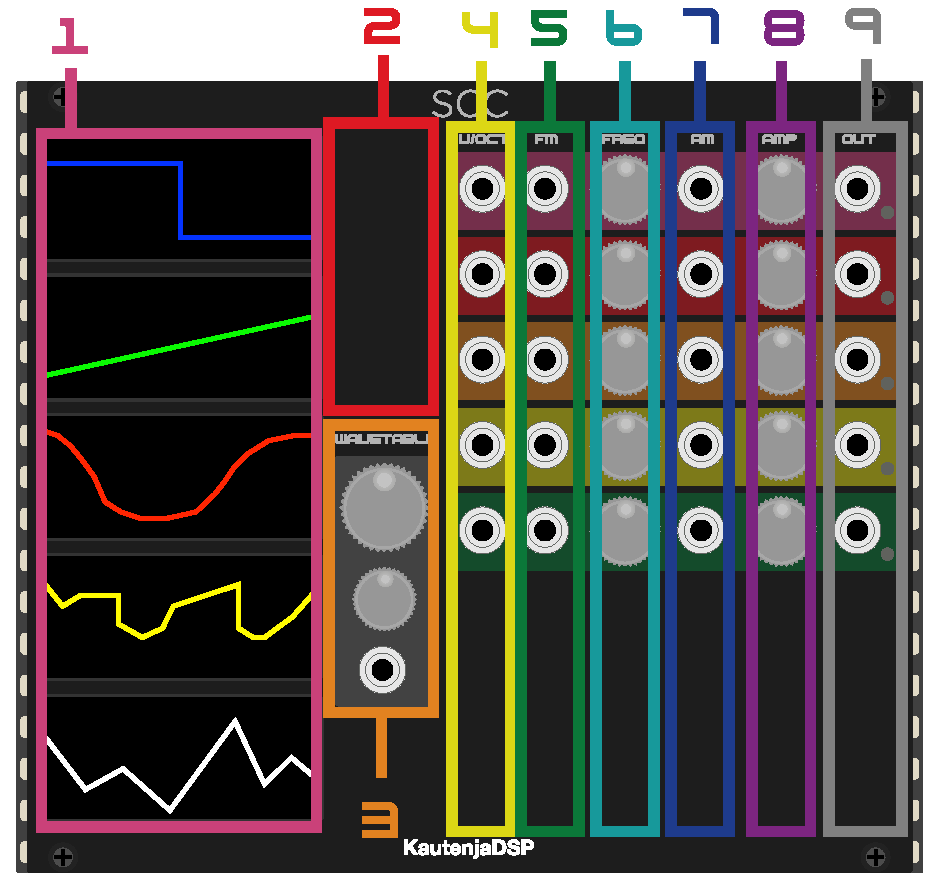
\includegraphics{SCC-Manual}
\end{figure}

% \begin{enumerate}
%   \item Coarse frequency control over the four oscillators.
%   \item $V$/Octave inputs for pulse1, pulse2, and triangle waveform generators.
%   \item linear CV frequency modulation for pulse1, pulse2, and triangle waveform generators.
%   \item Pulse width selector. Chooses between four duty cycles: $12.5\%$, $25\%$, $50\%$, and $75\%$.
%   \item CV LFSR gate, high at $2V$. Holds the LFSR generator as long as the input voltage is $>2V$.
%   \item Period of randomness $\in [0, 15]$ for the noise generator. See \url{https://wiki.nesdev.com/w/index.php/APU_Noise} for approximate frequency and pitch mappings.
%   \item Channel outputs, ${\approx}10V_{pp}$.
% \end{enumerate}

% -------------------
% MARK: References
% -------------------

\clearpage
\renewcommand\refname{References \& Acknowledgments}
\nocite{*}
\bibliographystyle{apalike}
\bibliography{references}

\end{document}
